\documentclass{article}

% if you need to pass options to natbib, use, e.g.:
%     \PassOptionsToPackage{numbers, compress}{natbib}
% before loading neurips_2021

% ready for submission
\usepackage[preprint]{neurips_2021}

% to compile a preprint version, e.g., for submission to arXiv, add add the
% [preprint] option:
%     \usepackage[preprint]{neurips_2021}

% to compile a camera-ready version, add the [final] option, e.g.:
%     \usepackage[final]{neurips_2021}

% to avoid loading the natbib package, add option nonatbib:
%    \usepackage[nonatbib]{neurips_2021}

\usepackage[utf8]{inputenc} % allow utf-8 input
\usepackage[T1]{fontenc}    % use 8-bit T1 fonts
\usepackage[colorlinks=true]{hyperref}       % hyperlinks
\usepackage{url}            % simple URL typesetting
\usepackage{booktabs}       % professional-quality tables
\usepackage{amsfonts}       % blackboard math symbols
\usepackage{nicefrac}       % compact symbols for 1/2, etc.
\usepackage{microtype}      % microtypography
\usepackage{xcolor}         % colors
\usepackage{graphicx}

\bibliographystyle{abbrvnat}

\title{Analysis of Remote Work Data}

% The \author macro works with any number of authors. There are two commands
% used to separate the names and addresses of multiple authors: \And and \AND.
%
% Using \And between authors leaves it to LaTeX to determine where to break the
% lines. Using \AND forces a line break at that point. So, if LaTeX puts 3 of 4
% authors names on the first line, and the last on the second line, try using
% \AND instead of \And before the third author name.

\author{%
  Manuel Rauschenberger\\
  Matrikelnummer 3609505\\
  \texttt{manuel.rauschenberger@student.uni-tuebingen.de} \\
  \href{https://github.com/mrauschenberger/datlit2022proj}{git repo}
}

\begin{document}

\maketitle

\begin{abstract}
I'm planning to use the \href{https://salaries.freshremote.work/download/}{collected remote work salaries data} to first make a choropleth (or two), as suggested, and then to do some statistical analysis (ANOVA) to find something out about the differences in salary earned depending on factors like company size, location or amount of work done remotely.
\end{abstract}

\section{Looking at the Data}
Since this dataset is updated from time to time, I will use the data I downloaded on the 1st of February, 2022, to write this report.
It consists of 2451 entries of salary data from the years 2020 and 2021, containing information, among other things, about the size and location of the company they worked for, their residence location and the amount of work done remotely, which is categorized as follows: A \texttt{remote\_ratio} of '0' means that less than 20\% of the work was done remotely, '100' means more than 80\% was done remotely and the rest goes under '50'. \\

\begin{table}[h!]
  \caption{One example entry from the dataset.}
  \label{sample-table}
  \centering
  \scriptsize
  \begin{tabular}{llllll}
  \toprule
	index & work\_year & experience\_level & employment\_type & job\_title & salary  \\
	\midrule
	1234 & 2020 & SE & FT & Security Engineer & 148000         \\
	\midrule \midrule
	salary\_currency & salary\_in\_usd & employee\_residence & remote\_ratio & company\_location & company\_size \\ \midrule
	USD & 148000 & US & 50 & US & M \\
	\bottomrule            
  \end{tabular}
\end{table}

It should be noted that the categories in this dataset are often quite unbalanced; looking at the amount of work done remotely, a majority of 1708 have stated that they did most of their work remotely, another 725 have worked partially remotely and only 18 fall under the category with 
less than 20\% of the work done remotely. \\
The largest amount of data comes from people living in the United States or working for a company based in the US, with 1321 participants stating that they work for a US-based company, and 1194 stating they live there. On the other hand, we have for example only one person from Cyprus in this dataset and only one person indicating they work for a company based in Afghanistan. \\
This is something to keep in mind of course, when looking at the following visualization and further analysis of the data. 

\section{Visualizing the Data}
Since there are two interesting geographical properties present in the data, namely the location of the company one worked for and the location of one's residence, I have decided to make two choropleths based on each of these properties. I have used the \texttt{geopandas}-package \citep{kelsey_jordahl_2021_5573592} for this purpose.

\begin{figure}[h!]
  \centering
  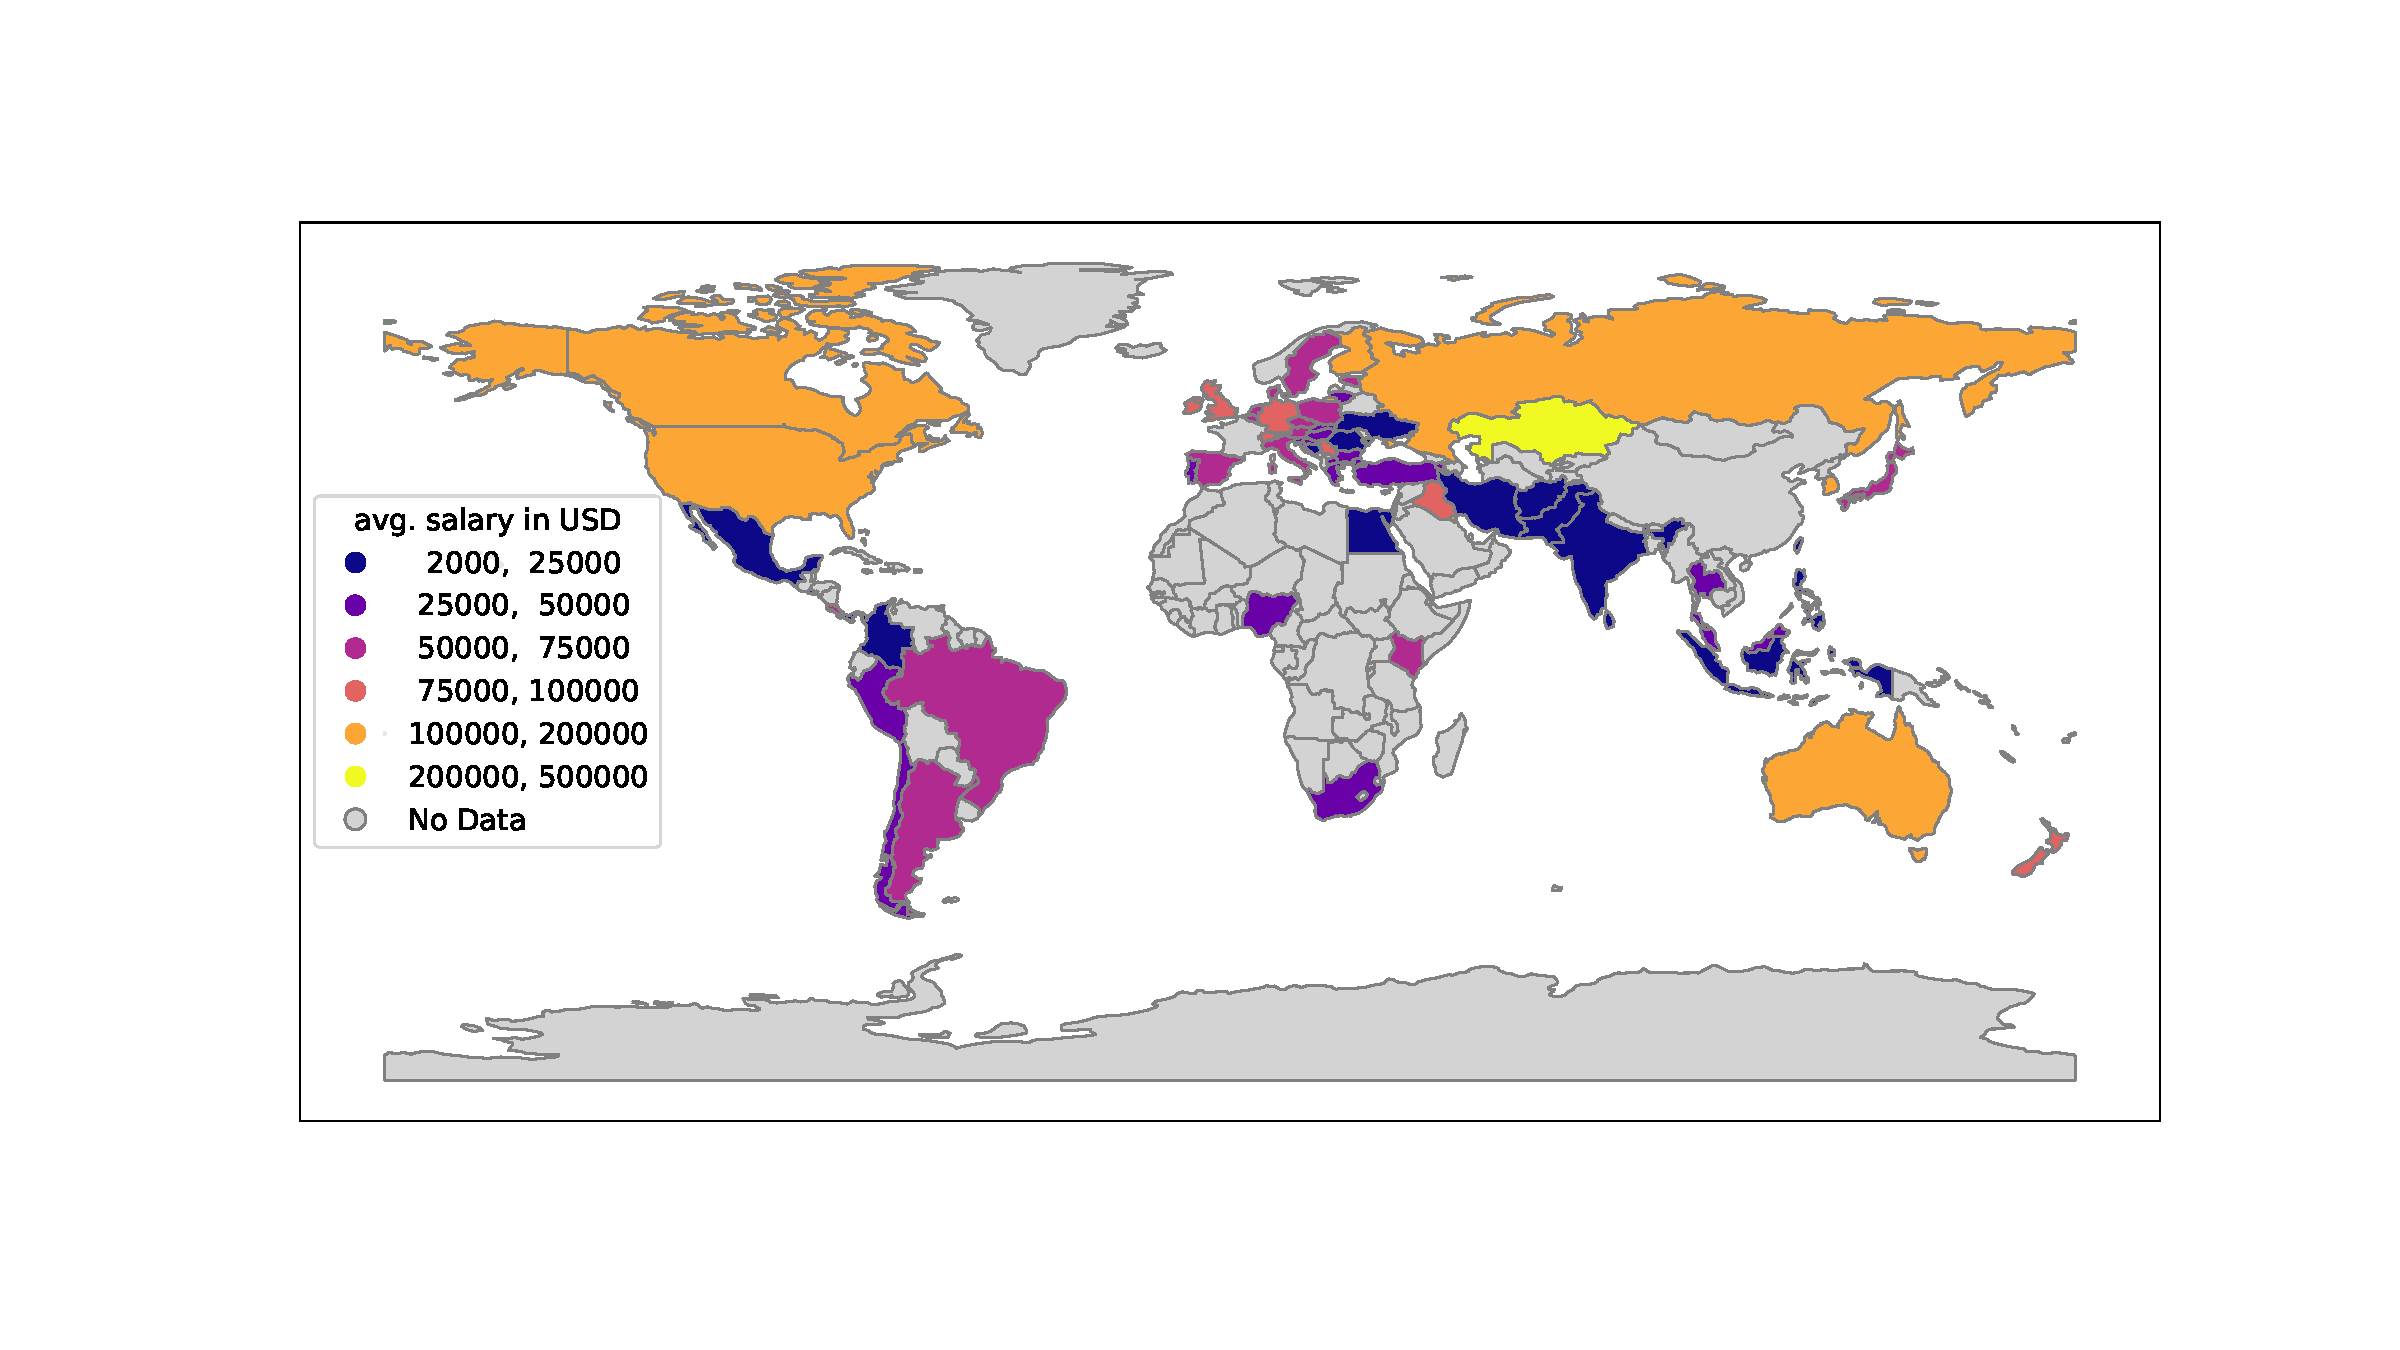
\includegraphics[scale=0.38]{fig/salaries_company_loc.pdf}
  \caption{Here we see the average salary in (US-Dollars) based on the location of the company they worked for.}
\end{figure}

As we can see, the highest average salaries are being paid by companies based in the USA, Canada, Russia, Australia, Finland, South Korea and, interestingly, Kazakhstan. Here I should note that this 'average' in Kazakhstan comes from just one person in the dataset, who lives in and works for a company in Kazakhstan and states to have a salary of 500.000\$. \\
For companies based in Germany and the rest of Europe, salaries seem to be a bit lower generally.

\begin{figure}[h!]
  \centering
  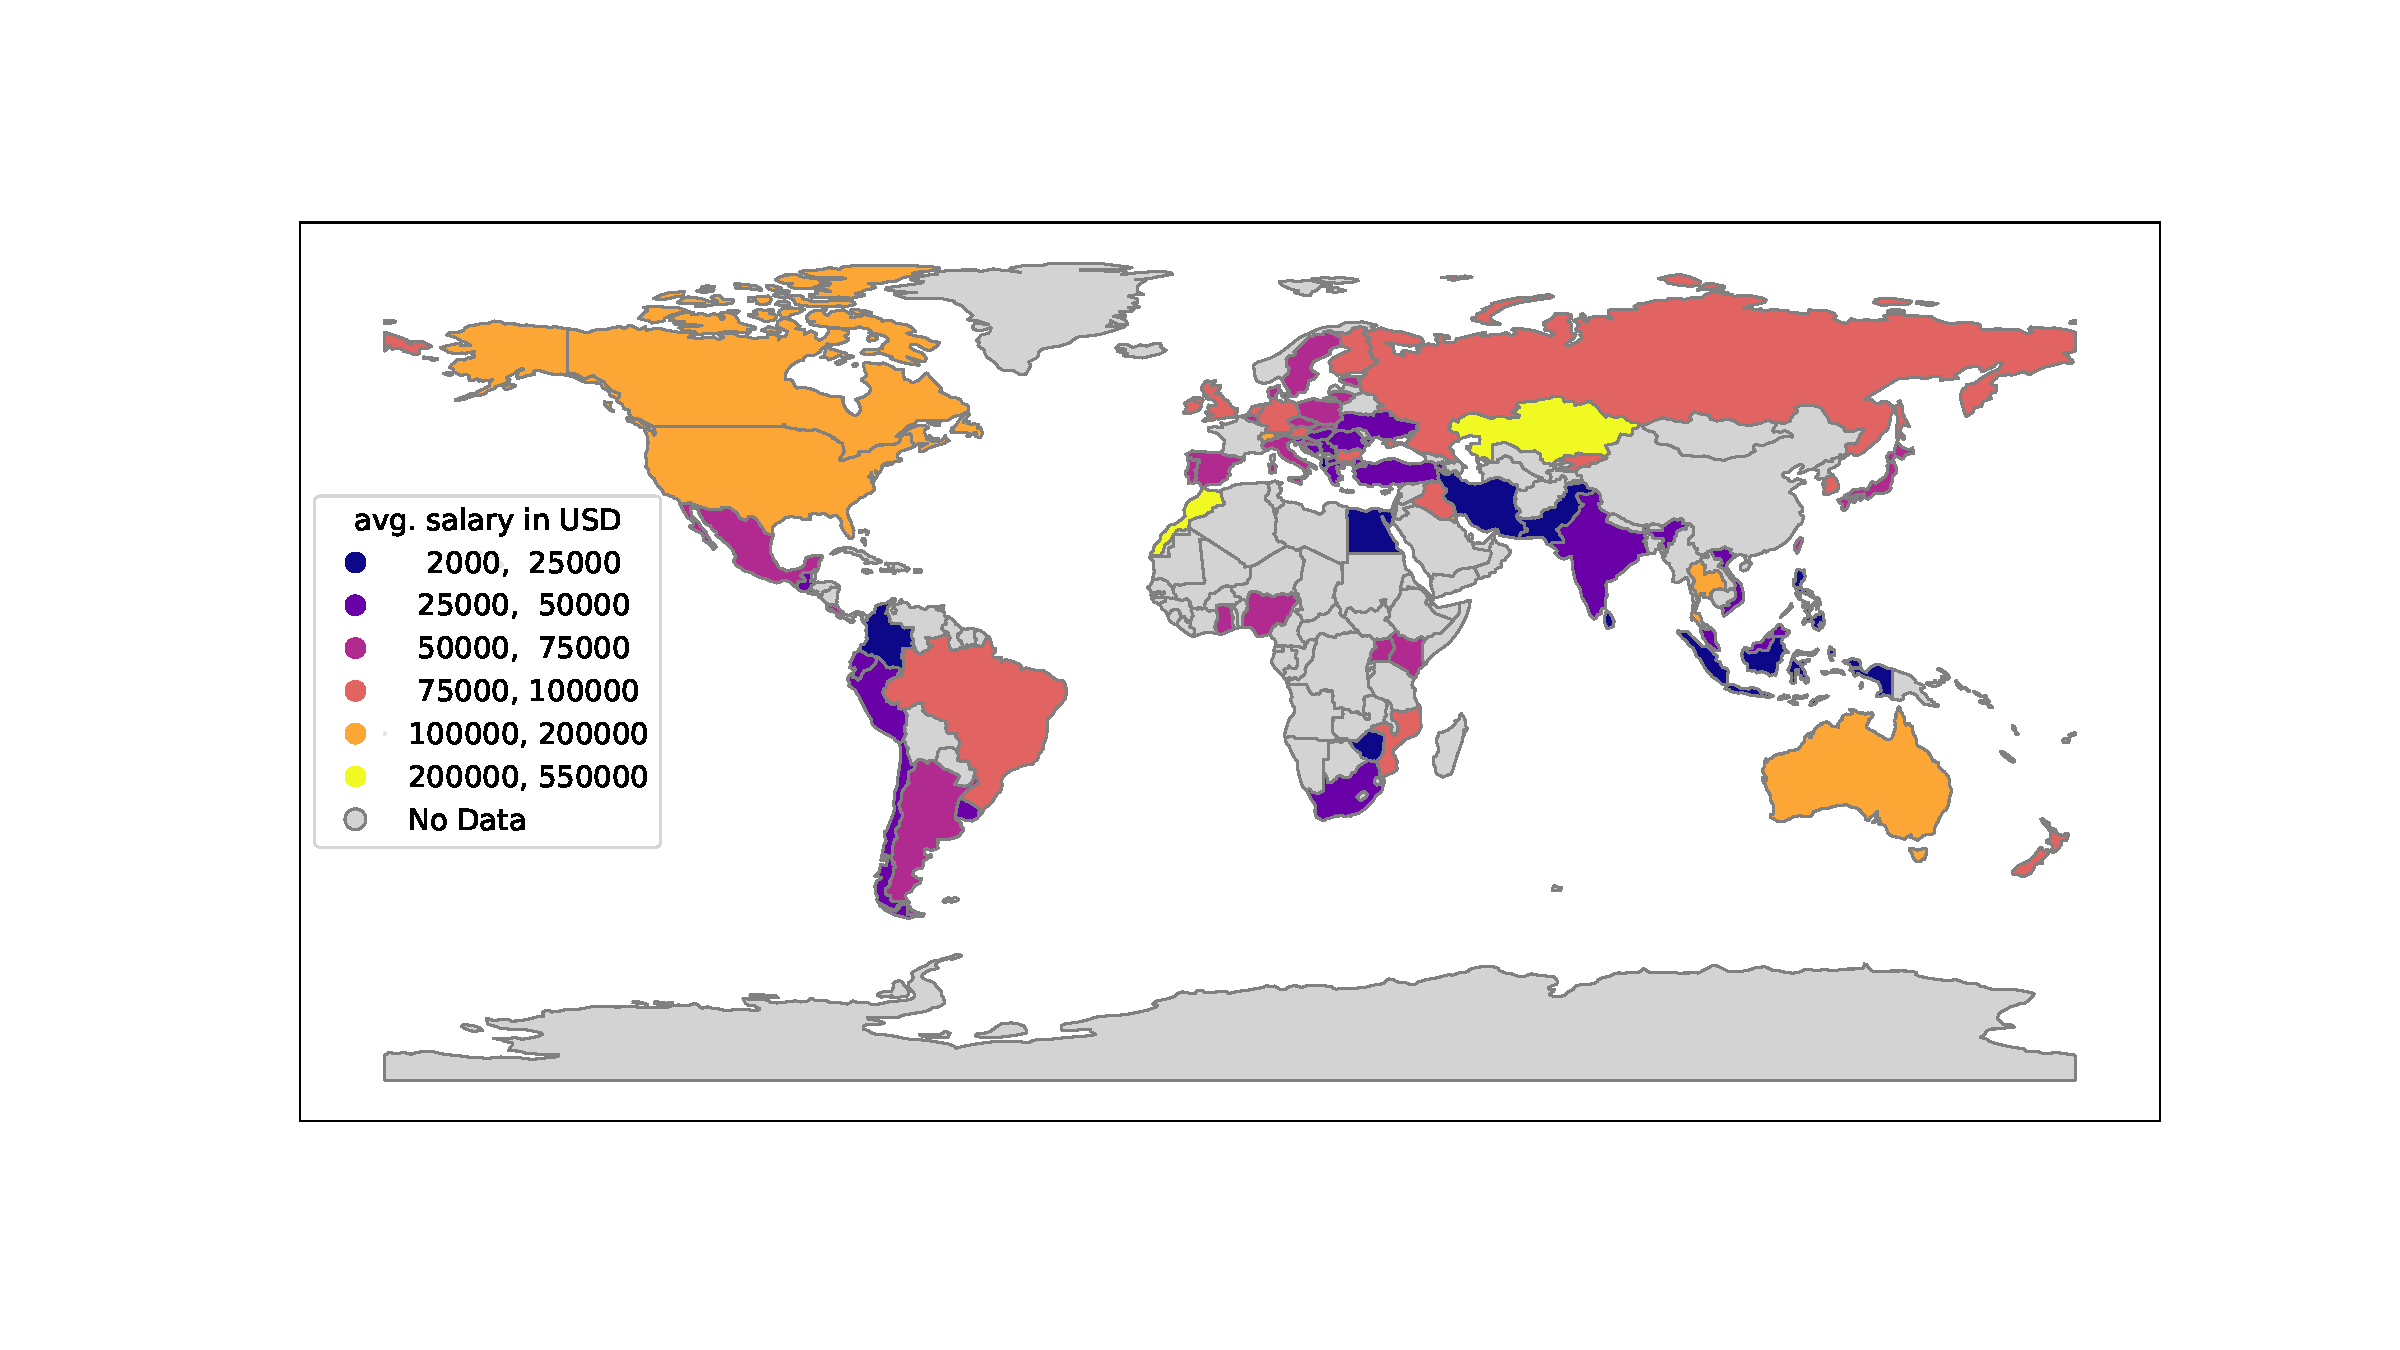
\includegraphics[scale=0.38]{fig/salaries_employee_loc.pdf}
  \caption{And here we have the average salary (in US-Dollars) based on the location of the residence of the employees.}
\end{figure}

The second Choropleth detailing the average salaries based on the residence of the employee generally looks rather similar to the one based on company location. This is of course to be expected, given that most people working for a company usually also live in the same country.

\section{Analyzing the Data}
I would like to find out if there is a difference in the salary means for different amounts of work done remotely. For this purpose I will conduct an ANOVA hypothesis test \citep{ANOVA}, with the null hypothesis $H_0$ being that salary means are equal among the three different groups categorizing remote work. \\
The requirements for this test are:
\begin{itemize}
\item That we have random, independent samples, which is fulfilled here.
\item That for each group, the variable under consideration is normally distributed; we will have to check for that.
\item That the standard deviations of the variable under consideration are the same for all groups; this we also need to verify.
\end{itemize} 
To see if the second requirement is fulfilled, we can look at a normal probability plot (Q-Q plot) for each grouped variable to see if the data points fall on a line. Well, for this dataset this isn't quite the case, partly because we have some outliers with much larger than average salaries. We will note that this requirement isn't perfectly fulfilled.

\begin{figure}[h!]
  \centering
  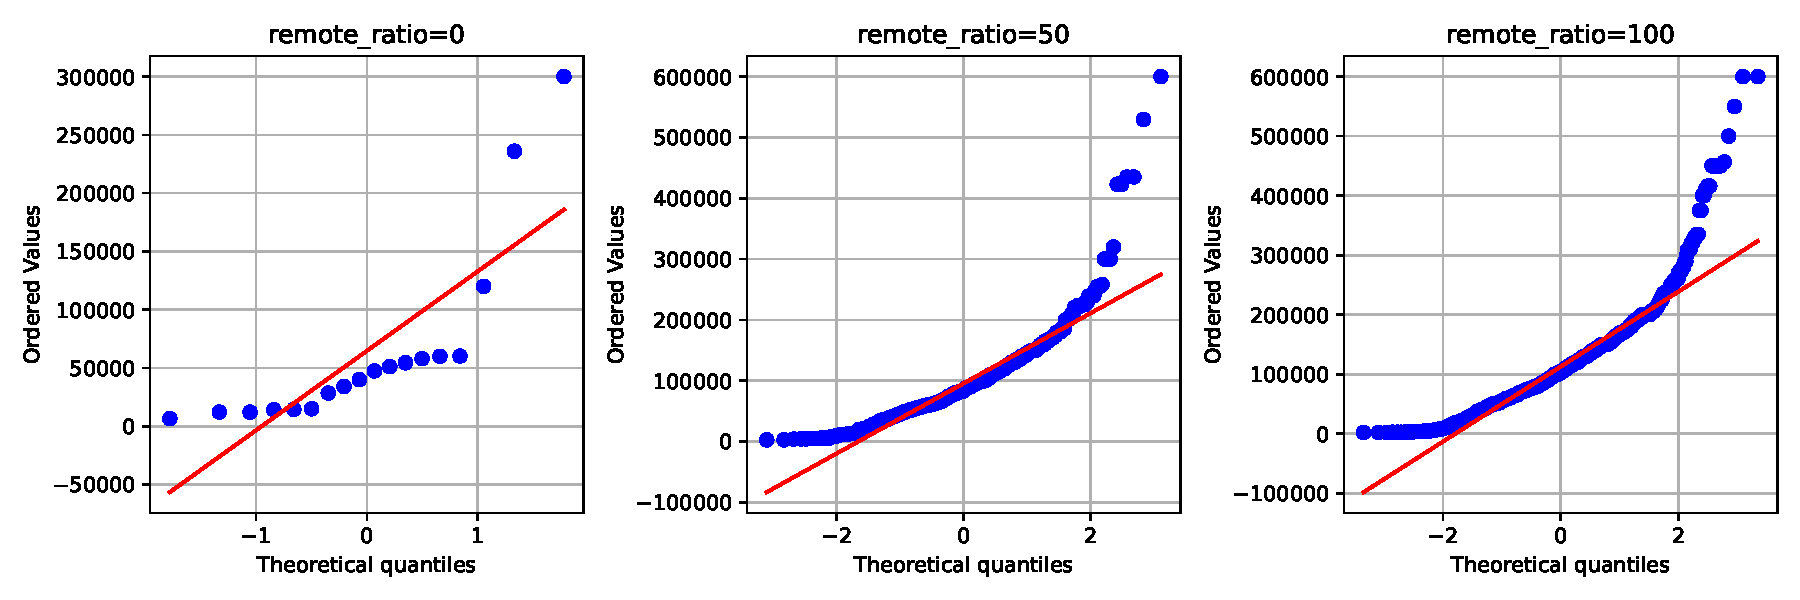
\includegraphics[scale=0.50]{fig/probplot.pdf}
  \caption{Q-Q plots for the three different groups detailing the amount of work that was done remotely. In this plot, the data points are normally distributed if they fall on a straight line.}
\end{figure}

To check the last requirement, we can look at the ratio of the smallest and largest standard deviation. If this ratio is less than 2, we can consider the requirement as fulfilled. In this case, the ratio is $1.266254$, so that's fine. \\ \\

Now that we have seen that the requirements for the ANOVA hypothesis test are (roughly) fulfilled, we can perform the test. Again, our null hypothesis is that all mean salaries are the same among the different categories of remote work amount, so we can check if we can reject this hypothesis, which would mean there is a difference in the mean salaries. As significance level, I will choose $\alpha = 0.05$.

\begin{table}[h!]
  \caption{Result of the one-way ANOVA hypothesis test.}
  \label{sample-table}
  \centering
  \begin{tabular}{cllllll}
    \toprule
    Source of Variation & SS & df & MS & F & p-value & F crit \\
    \midrule
    Between Groups & $1.7962 \cdot 10^{11}$ & 2		& $8.9812 \cdot 10^{10}$ & 20.884 & $1.0152 \cdot 10^{-9}$ & 3.6944 \\
    Within Groups  & $1.0527 \cdot 10^{13}$ & 2448	& $4.3004 \cdot 10^{9}$ & & & \\
    Total     &      $1.0707 \cdot 10^{13}$ & 2450	& $4.3702 \cdot 10^{9}$ & & & \\
    \bottomrule
  \end{tabular}
\end{table}

The result of the test gives us a $p$-value of $1.0152 \cdot 10^{-9}$, which is clearly smaller than our significance level, therefore we can reject the null hypothesis. So we find that there is a significant difference in remote work salaries, based on the amount of work done remotely. \\
This result is somewhat surprising to me, since my expectation was that there shouldn't really be a big difference to be found here. After all, the salaries of all the people who, during the pandemic, had to work remotely more often, shouldn' really have changed much. But of course one also needs to once again note that there are only 18 samples available for the 'no remote work' group, which just isn't enough to perform precise statistical analysis. \\ \\
But since there are also other features available in the data, I wanted to try a two-way ANOVA as well, using the \texttt{remote\_ratio} and \texttt{company\_location} categories. This is implemented in the \texttt{statsmodels}-package \citep{seabold2010statsmodels} and provides another interesting result.


\begin{table}[h!]
  \caption{Result of the two-way ANOVA hypothesis test.}
  \label{sample-table}
  \centering
  \begin{tabular}{cllll}
&						SS	&		df 		&F 			&p-value \\
\midrule
C(remote\_ratio) &		$6.264463 \cdot 10^9$ &	2.0 	&1.001624 &	$3.674374 \cdot 10^{-1}$ \\
C(company\_location) &	$3.094188e \cdot 10^{12}$ &	71.0 	&13.936040 &	$1.314224 \cdot 10^{-131}$ \\
Residual 		&		$7.433241e \cdot 10^{12}$ &	2377.0 	& & \\
    \bottomrule
  \end{tabular}
\end{table}

Here the $p$-value for the \texttt{remote\_ratio} feature is actually much larger, with $p = 0.3674374$, which would mean that this feature is actually not significant at all. The significant feature is in fact the location of the company, with a $p$-value of $p = 1.314224 \cdot 10^{-131}$. \\

So in the end, we really can't say from this data alone, if there is a difference in salaries based on the amount of work done remotely. It would of course help to have more data, especially in the 'no remote work' group, so that the groups aren't as unbalanced, but perhaps there also just isn't a significant result to be found there.

\bibliography{Literatur}

\end{document}
